\documentclass{l4proj}

%Packages
\usepackage{natbib}
\usepackage{graphicx}
\usepackage[normalem]{ulem}
\useunder{\uline}{\ul}{}
\usepackage{pdflscape}

\begin{document}
\title{Augmented Reality Android Gym App}
\author{David Benicek 2073063b}
\date{\today}
\maketitle

\begin{abstract}
Something will go here.
\end{abstract}

\educationalconsent
%
%NOTE: if you include the educationalconsent (above) and your project is graded an A then
%      it may be entered in the CS Hall of Fame
%
\tableofcontents
%==============================================================================

\chapter{Introduction}
\pagenumbering{arabic}
\section{Motivation}
Frequent exercise and a healthy lifestyle have recently become an integral part of the western culture. Indeed, last year in America more people have exercised on a regular basis then ever before \cite{riffkin_so_2015}. As people begin to adopt this new and healthy lifestyle, it is immediately obvious that there are two distinct periods during which there seems to be a lack of coherent information. These are at the very beginning when a person begins to exercise for the first time and when a person begins to plateau and starts to experience diminishing returns for their workouts due to a lack of variation in their routine. It is important to note that a lack of coherent information does not necessarily mean a lack of data but instead a lack of a singular consensus in the midst of conflicting information, fad diets, ill-informed advice and 'bro science'. Therefore, it seems that there is a need for a singular portal to which both beginners and experienced gym goers alike can refer to for information regarding exercise.  

\section{Aim} \label{sec:aim}
Tackling the entire topic of fitness in one application would be extremely difficult, if not impossible. Due to this we are going to narrow down the focus and seek to add value to users while they are in the gym. The aim of the application will be to help users understand how to use gym equipment, suggest a range of exercises that can be carried out on a given piece of equipment and demonstrate how to perform the exercise with correct and safe form. 

One of the main goals of the app is for it to be responsive to the user's environment and heavily interactive so that the user has an immersive experience. An immersive experience will keep users engaged with the app however there is a balance to be drawn here. Since the gym is a potentially dangerous environment, the design of the app must make sure that users do not loose track of their surroundings completely. One possible way of striking this balance is through augmented reality (AR). AR would allow us to give a somewhat immersive experience by super imposing realistic human models on the device's screen without the need for a completely virtualized reality. Similar applications of AR have been trialed in education, construction, sports and medicine to various degrees of success. A review of literature regarding previous work done with AR can be found in section \ref{sec:litrew}.

\section{Outline}
In this document we are going to explore the different steps taken in the development of the augmented reality gym app. First, we will review relevant literature in order to be able to make informed decisions concerning requirements and constraints. Requirements elicited from discussions with the Glasgow University Sports Association (GUSA) will also be review and summarized. Following, will be a discussion of the possible designs of the app from both a user experience and user interface aspect. Later we will go trough the steps in implementation and testing, outlining the procedure and any major problems along the way. Finally, we will draw the document to a close with a conclusion, followed by an evaluation, where we will address to what extend the main objectives of the project were achieved and reflect on what could have been done differently for future reference. 

\chapter{Requirements}

\section{Requirements Elicitation}
\subsection{Review of previous work} \label{sec:litrew}
The term 'augmented reality' was coined by Tom Caudell, a Boeing researcher in 1990 \cite{rauterberg_history_2002}. Caudell first envisioned augmented reality as transparent screens that would be used to display complicated plans and designs. AR has evolved tremendously since the 1990s and with it so has it's definition. In order to understand augmented reality we first have to address the concept of mixed reality. Mixed reality is the overarching concept of blending the real and virtual worlds \cite{milgram_taxonomy_1994}. Within the field of mixed reality there are many branches which lie on a spectrum between a non-manipulated, real environment and a fully digital environment created in virtual reality. The spectrum can be see in figure \ref{fig:ar-spectrum} and it is important to note that immersion increases as we move to the right from the real environment to the virtual environment. Augmented reality sits in the center left of the spectrum and can be broadly defined as "technologies that project digital materials onto real world objects"\cite{cuendet_designing_2013}. Importantly, augmented reality integrates "3D virtual objects ... into a 3D real environment in real time"\cite{azuma_survey_1997}. The added virtual content is obviously superimposed and the distinction between real and virtual is clear, unlike with other technologies further to the right on the spectrum. For example, on the extreme right of the spectrum is virtual reality, which fully replaces the real world with computer generated scenes and aims to mimic the real world \cite{tamura_mixed_2001}. This paper is only concerned with augmented reality since it provides just enough immersion to exploit phenomenon such as situativity and yet, does not cause the user to be completely absorbed into the application, nor does it require additional equipment. 

\begin{figure}[h]
\centering
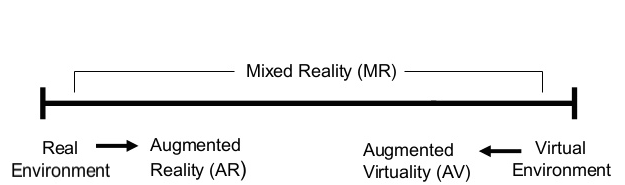
\includegraphics[scale=1]{images/ar-spectrum.png}
\caption{A spectrum overview of mixed reality technologies (Milgran 1994)}
\label{fig:ar-spectrum}
\end{figure}

AR has been used in a number of disciplines, ranging from medicine to entertainment to construction.\cite{azuma_recent_2001}. It seems that there has been no previous research done on the possible application of AR in the fitness sector and therefore we will draw on insights from other applications of AR. We will especially focus on pedagogical applications of AR with the hope of drawing parallels between teaching a class and instructing users to perform exercises in the gym. 

The use of AR in classrooms has been trialled by many and there is plenty of research evaluating it's effectiveness. AR in classrooms has been widely used in the past on desktop machines \cite{iordache_comparison_2009} but it's true power has only been unleashed recently, as the shrinking of technologies has allowed AR to migrate from desktop to mobile devices \cite{squire_augmented_2007}. Squire and Klopfer studied four different groups of students using an AR game in which students took on the role of environmental detectives. One of the main advantages of AR highlighted in their study was the ability to trigger the recollection of preexisting knowledge \cite{squire_augmented_2007}. "Learning is contextual" \cite{liestol_learning_2011} and so, by placing students in a familiar environment, they are likely to recollect what they previously learnt in the same location. This is supported by the pedagogical psychologist Greeno, who put forward the theory of situativity, arguing that immersing oneself in the context of a situation aids with its understanding and recollection of previous relevant information\cite{greeno_situativity_1998}. Dede has studied full virtual reality and has noted the positive effects of immersion on the transfer of knowledge from theory into practice in the real world\cite{dede_immersive_2009}. Importantly, according to Dede "lesser degrees of immersion can still provide situated learning" and all the benefits that come with it\cite{dede_immersive_2009}. Situativity is an extremely powerful tool and the gym application must exploit it. Ergo, using situativity should be one of the requirements for the application. By simply by placing users in the correct environment, they will have a higher chance of recalling and learning the correct form of an exercise. All in all, the advantage of situativity as well as the evidence that suggests AR is an effective way to visualise information and instructions \cite{squire_augmented_2007} suggest it is a suitable technology for teaching and for use in the gym application.

\textbf{Requirement I:} \textit{"Exploit situativity through location based interaction"} \label{requirement_I}


Iulian Radu expanded on the initial research of using of AR in classrooms. Similarly to Squire and Klopfer, Radu noticed a number of specific positive impacts that AR can have on learning. In Radu's experiment, AR increased understanding and the long-term retention of taught content as well as the student's motivation\cite{radu_why_2012}. Unfortunately, Radu also noticed some usability difficulties and fluctuating levels of understanding between students \cite{radu_why_2012}, hinting at the fact that design and usability are key in AR applications. Others, such as Liestøl, have realized the possible difficulties in adopting AR in the classroom but Liestøl stated that "the threshold for entering this technology is not insurmountable - it is actually relatively easy"\cite{liestol_learning_2011}. Indeed, the benefits that AR brings, such as improved learning, higher retention and motivation are extremely positive but they do come at a cost. The initial adoption of AR may bring with it some issues but if resolved, the prospects of AR are truly impressive. In  pedagogy, most teachers would need to create their own AR application, or use one that is specifically targeted at their syllabus and at what they are trying to teach students, however, in the context of the gym app, there is no need for each individual user to re-create the app since the exercises they are trying to learn are uniform. This removes a significant barrier to the use of AR in the gym and all that is left to do is for the user to familiarize themselves with the AR app - just as they would with any other non-AR mobile application. 

\textbf{Requirement II:} \textit{"Ensure the application is usable in any environment and with any brand of equipment"}  \label{requirement_II}

Yet another advantage of mobile AR applications is that they allow the users to move around the scene and explore different angles and perspectives of the rendered object, thus catering to a more dynamic and interactive learning experience\cite{fitzgerald_augmented_2013}\cite{dede_immersive_2009}. Kerawalla et al. carried out an experiment where AR was assessed against other, more traditional, methods of teaching a class about the solar system\cite{kerawalla_making_2006}. In total, 133 children grouped in different classes attended the experiment. Each class was split into three groups and each group was then run through two sessions using different teaching methods. There were four variations to the teaching styles: Teaching using AR by a teacher who is an expert in AR, using AR by a teacher who had no prior experience with AR, using the classic lecture and bookwork combination and finally using the BBC ReviseWise website where kids work independently at the computer. The debate during class was analysed and the teachers were interviewed a few days after the class occurred. One of the main outcomes of the experiment was that teachers saw the value in AR making "traditionally inaccessible subject matter available to the children"\cite{kerawalla_making_2006} and thus enriching their learning experience. In the study, space was the inaccessible subject but in our context AR will be used to substitute a fitness instructor. Kerawalla et al. did not go as far as to assess the amount of information kids learned during the AR session in comparison to the sessions taught in a traditionally style but one teacher highlighted that thanks to using AR, a student "can see that picture in his head rather than just being told it, or like with a globe and a torch ... having to work out what stands for what"\cite{kerawalla_making_2006}. All in all, the teachers found that AR made "the  subject  matter  accessible  and real". Using AR to demonstrate how things work and replacing old, mundane methods seemed to be very effective and is also one of the requirements of the gym application.  

\textbf{Requirement III:} \textit{"Eliminate the need for an instructor to demonstrate an exercise"}  \label{requirement_III}

One of the main issues with AR technology in general is alignment \cite{sood_pro_2012}. Object recognition, especially on mobile devices, does not yet have the needed fidelity to be able to distinguish the same object in different variations. For example, object recognition could be used to recognize a bench in the gym however, it will only ever be able to recognize that specific type of bench. In a different gym, with different benches or even with the same bench but different lighting, shadows and perhaps colour, object recognition will do us no good. One possible solution, proposed by Rekimoto and Ayatsuka is to have visual tags on the objects and use these to identify them \cite{rekimoto_cybercode:_2000}. We can group objects that fall in the same category by giving them the save tag and placing it in the correct area. We then use image recognition to recognize the tag and use it as an anchor for our augmented reality overlay. This solved the issue of alignment because we don't need to know where the object we are projecting the visualization onto starts and end, we simply use the size and orientation of the marker to draw the visualization. Then, by constantly tracking the position and size of the visual tag, we can move and size our augmentation accordingly.

\textbf{Requirement IV:} \textit{"Ensure that there are no issues with alignment or target recognition"}  \label{requirement_IV}

Having a virtually augmented layer in the users view gives a new interface for human computer interaction. Balog et al. used AR glasses and a 'paddle' to point at and select virtual objects as a part of a class room exercise. There were several issues identified in their research, most important were the inability to select every element due to overlapping object, maneuverability, the paddle blocking the view of the user and a lack of feedback\cite{balog_augmented_2007}. Despite some of the shortcomings, a group of 32 students scored the AR exercise as exciting (4.16 on a 5 point scale) and gave scores of 4.38 and 4.34 respectively for understanding the lesson and readability of presented information\cite{looser_evaluation_2007}. On the other hand, interacting with the virtual objects using the 'paddle' was ranked lower, at only 3.06\cite{balog_augmented_2007}, Looser et al. also experimented with different input methods, testing selection with a virtual hand and with two methods of using virtual pointers\cite{looser_evaluation_2007}. Both uses of pointers performed poorly, with error rates deviating around 45\%\cite{looser_evaluation_2007}. The virtual hand performed much better but still suffered from a 20\% miss rate\cite{looser_evaluation_2007}. These findings suggests it is better to choose  more traditional methods of user interaction instead of opting for a virtual interface. Based on this, the gym application will implement a touch screen interface with standard on-screen buttons rather than using a fully augmented virtual interface. 

\textbf{Requirement V:} \textit{"Create an easy to use on-screen graphical user interface"}   \label{requirement_V}


Perhaps the most important issue when creating a phone app in general and an AR app in particular is the issue of attention tunneling \cite{radu_why_2012} \cite{biocca_attention_2007}. Attention tunnels, such as oncreen indicator that point the user in the correct direction have previously been used with impressive sucess\cite{biocca_attention_2007}. In one experiment, attention funnels increased "the consistency of the user’s search by 65\%,  increased search speed by 22\%, and decreased mental workload by 18\%" \cite{biocca_attention_2007}. Clearly attention funnels can extremely useful but since using AR is a relatively immersive experience, we must take care to draw the users attention to the appropriate stimulai and objects in order for them to not completely loose track of their environment - especially in the gym, which is a potentially dangerous environment. Biocca et al. have pointed out issues with attention funneling in mobile interfaces in general, stating that "the attention demands of current interfaces such as cellular phones and PDAs may play a significant role in automobile accidents". Some AR applications such as Pokemon Go have solved the issue of attention tunneling through pop ups that remind the user to stay aware of their surroundings \cite{hollister_drivers_2016}. A similar approach should be adopted in our application to ensure the users safety and must be one of the high priority requirements.

\textbf{Requirement VII:} \textit{"Avoid users from becoming fully immersed into the application"}  \label{requirement_VI}


\subsection{Meeting with GUSA}
When developing an app of any kind it is important to consider how you are going to market and distribute the finished product. This question is particularly interesting in our context because the app needs some real-life components (markers) to work and therefore needs to be pitched to both daily users and gym owners. One of the first steps that I carried out, before doing much research into technologies and development was to arrange a meeting with the Glasgow University Sports Association (GUSA). I pitched my idea to the president of GUSA in an email and was able to arrange a meeting both with GUSA president and the Sport Development Manager at Glasgow University. The meeting 	was held on the 26th of July 2016 and yielded a number of interesting requirements and points of discussion, many of which I had not previously considered. 

One point of discussion was the issue of liability. The main goal of the app is to demonstrate what perfect form of an exercise looks like, however there are conflicting views as to what 'perfect' form for an exercise is. Most of the times there will be a theoretical ideal motor pattern to lift the most weight efficiently, however when a user tries to recreate this, they might be put in a compromising position. Take, for example, the deadlift (picking up a bar from the floor and finishing in a standing position with the bar mid thigh). Within the app, we may demonstrate that the safest starting position is from a half-squat where the thighs make a 25° angle with the floor. This may indeed be the safest position for someone with a perfectly proportionate body, but if somebody has shorter arms and longer legs, they may need to squad down further to reach the bar and be in a strong position. If such a user were to follow our instructions too closely they may round their back in order to reach down to the bar and end up hurting themselves. If a user was so inclined, they could blame the app for providing unsafe instructions to them. A potential solution would be to show a disclaimer within the app or during app launch that notifies the user that all demonstrations of form are approximate and that the user should contact an expert if they are unsure how to properly and safely perform an exercise. If a user is clearly made aware that the demonstrated form for each exercise is only approximate and shows what the creators deemed most efficient, then there should be no liability issues. 

\textbf{Requirement VII:} \textit{"Show theoretically perfect form and notify user of any dangers"} \label{requirement_VII}

GUSA was cautious about how the app is going to be distributed and marketed since they are themselves working on a designated GUSA app and are also pushing the LifeFitness app to their customers. The main concern was that by having too many apps marketed in the gym, customers would be overwhelmed and end up using none of the apps. It was decided that in order to solve this dilemma, my app would not be distributed by GUSA nor will it have any relation to GUSA. Instead the Glasgow University gym will simply be an environment for testing. 

\section{Acceptance Criteria}
Setting goals without a concrete strategy to monitor them usually results in wasted time. In this section we are going to outline how we will measure success of the different requirements laid out in the previous section. These acceptance criteria will be refereed to throughout the project to track progress and at the conclusion of the project to evaluate the end product. 


\begin{table}[]
\centering
\resizebox{\textwidth}{!}{%
\begin{tabular}{llll}
Requirement Number & Requirement Text                                                                    &                                                                                                     & Acceptance Criteria                                         \\
I                  & Exploit situativity through location based interaction                              & Is the app usable in the gym?,Is there utility from using the app in the gym as opposed to at home? & User feedback                                               \\
II                 & Ensure the application is usable in any environment and with any brand of equipment & Does the app work anywhere and with any brand of equipment?                                         & Test app with multiple manufactures/in multiple environment \\
III                & Eliminate the need for an instructor to demonstrate an exercise                     & Can users use the app and gain knowledge by themselves?                                             & User feedback                                               \\
IV                 & Ensure that there are no issues with alignment or target recognition                & Does the tracking work well?                                                                        & User feedback                                               \\
V                  & Create an easy to use on-screen graphical user interface                            & Do users understand how to use the app?                                                             & User feedback                                               \\
VI                 & Avoid users from becoming fully immersed into the application                       & Is there any way to avoid users getting sucked into the app?                                        & Observe users as they use the app                           \\
VII                & Show theoretically perfect form and notify user of any dangers                      & Are users aware of any possible dangers?                                                            & User feedback                                              
\end{tabular}%
}
\caption{My caption}
\label{my-label}
\end{table}

\chapter{Design}
\section{User Experience}
The quick brown fox jumped over the lazy dog.
The quick brown fox jumped over the lazy dog.
The quick brown fox jumped over the lazy dog.
The quick brown fox jumped over the lazy dog.
\section{User Interface}
The quick brown fox jumped over the lazy dog.
The quick brown fox jumped over the lazy dog.
The quick brown fox jumped over the lazy dog.
The quick brown fox jumped over the lazy dog.

\chapter{Implementation}
The development of an augment reality phone application sounds quite daunting at first. The image recognition, 3D object imaging and use of sensors and mathematical calculations to pivot the projected image are undoubtedly complex however, there are many libraries and tools that allow us for the abstraction of the complex and intricate work and allow us to focus on the core app development. Despite this, the initial learning curve to find, set up and get started with all the tools and technologies is quite steep. In order to make the process easier implementation will be broken down into three iterations which will build upon each other incrementally and allow for frequent feedback. In this section we are first going to explore the numerous tools used throughout the project, justify their selection and talk about how they are used. Later each of the three iterations will be examined and some of the major events, decisions and problems will be pointed out.

\subsection{Technologies used}
\subsubsection{Git}
One of the first tools that was set up as a part of the project was the Git version control system. Git is usually used in the open source community or within teams to allow easy integration between contributors. In our case Git is used to keep a backup of old versions of the project and to share the progress of the project with the project supervisor. There are many other version control systems such as SVN or Merculiar. Git was chosen due to my familiarity with it and due to the fact that in most cases it is an industry standard.
	
\subsubsection{Vuforia}
Vuforia is one of the many open source augmented reality libraries \cite{vuforia_getting_2016}. Vuforia provides an online interface where you can upload different images which are then analysed for specific feature patterns that are used for matching. For example figure \ref{fig:coca_cola_features} show the feature patterns of a CocaCola logo. A collection of such targets can be exported as a database and later used in Unity for matching using optical recognition \cite{rao_how_2015}.
\begin{figure}
\centering

\includegraphics[scale=1]{images/coca_cola_features.png}
\caption{Patterns of features on the CocaCola logo.}
\label{fig:coca_cola_features}
\end{figure}

Vuforia allows us to create markers but it is also a plugin for Unity and an SDK that is used in native Android code development \cite{rao_how_2015}.

\subsubsection{Unity}
Unity is a well known 3D cross-platform games engine that is widely used in the field. There are many other game engine alternatives, however, Unity was chosen due to it's seamless integration with Vuforia and MakeHuman. Unity also allows us to export into different platform native application and so, even though Android is out target platform it would be relatively easy to port the application over to an iOS device or Windows mobile. 

\subsubsection{MakeHuman}
MakeHuman is a humanoid modeling software that makes creating life-like humanoid	 figures very easy. MakeHuman has a simple interface which allows the users to customize and configure their character. Many open-source online forums are also dedicated to creating a large database of download-able body parts and clothing, enriching the variety of customization that MakeHuman provides.

\subsection{First Iteration}
The goal of the first iteration was to come up with a functioning prototype that would serve as a proof of concept regarding the different technologies and explore how best to achieve the desired objectives. 

\subsubsection{Logical Layout}
One of the first major issues encountered was concerning the logical layout of the application. The initial intention was to create the core AR functionality of the app in Unity and then export the project into Android Studio where I would create the other views such as the home screen, setting page etc. I spent a couple days setting up the environment, learning about app development for Android and following tutorials to acquaint myself with the tools. I was eventually able to export the Unity project, import it into Android Studio and build a home screen that would load on start up and allow the user to navigate to a camera view which would contain the AR part of the app. Unfortunately, whenever the user would switch between the two views the unity launch screen would show up. This is undesirable for two reasons. First, showing the launch screen slows down the use of the app as it introduces unnecessary latency. Secondly, showing a splash screen in-between two of the main views deteriorates the natural flow within the app since splash screen are usually shown on startup and could cause users to get confused about how to navigate between views. Furthermore, showing a seemingly random branded splash screen in the middle of the app takes away from the brand and united design that the app should have. 

In order to remedy the situation I tried a number of fixes. For example, I tried loading the camera view first on startup and then automatically switching to the home view once the splash screen loaded. While this did successfully show the splash screen on launch, it did not solve the problem because the splash screen would still show when switching onto the camera view. I also looked into modifying the automatically generated unity files to stop the splash screen showing up all together but in my research I found out this violates the Unity terms and conditions. In order to remove the splash screen legally I would need to upgrade to the professional version of Unity (TODO: Cite unity) which is not an option due to financial constraints of the project.

The solution arose organically as a result of me becoming more familiar with Unity. As I began building the user interface for the camera view I discovered that Unity has an inbuilt tool for creating interfaces and I could simply create a new scene in Unity which will then serve as the main menu. By attaching scripts to different components I can make the menu dynamic and add functionality. The only disadvantage with this approach that I will be forced to write the scripts in C\#, which I am not familiar with, as apposed to the originally intended language of Java, which I am proficient in. 

\subsubsection{Animations}
Animations are an important part of the app and are a representative part in it's design. A handful of exercises were available online for free from open-source sources however these are not enough. In order to provide a realistic representation of how the app would look when complete and to validate the development process, custom exercises must be created. The tool used to create the animations is Blender which provides a detailed and complex interface for professional animations. There are two main issues with creating animations. I have no previous experience with animating nor with BLender and so the complex interface was quite overwhelming at first. The learning curve was made worse by the fact that some of the key-bindings were, by default, overlapped because I was using a laptop which did not have a full numerical pad. Thus whenever I would try to switch view using the top row numbers, different bones would get copied making the animation jump back and forth. Reassigning the key bindings solved the issues however the learning curve was still significant.

Even once I was able to learn how to use Blender and how to animate, it was still difficult to know exactly what form exercises should have. In order to present an accurate and safe representation of each exercise I needed a point of reference. After some research I found that forms of exercises vary depending of sources. Rather than combining different sources and compromising on form, I decided to pick a single reputable source and base my animations on it.  I found that the database exercise on bodybuilding.com provides a varied range of exercises with plenty of description both in text and images making it a suitable choice. Even with a clear intention and method on how the animation should look and be made, the actual creation of the animations is time consuming, meaning that we have to limit the number of animations that we are going to be self-created.

\subsubsection{2nd Meeting with GUSA}
A second meeting with the president of GUSA took place on the 15th of November 2016 in order to discuss progress on the application and gather feedback from a de facto expert in the field. During the meeting I demoed the application and asked the president for his opinion on a number of design choices and possible features. At the time of the meeting the application was largely at a proof of concept stage. Consequently, the design of the application (as can be seen in figure \ref{fig:it1}) was temporary and much of the discussion during the meeting revolved around possible additional features that could be implemented in the future. 

\begin{figure}[h]
\centering
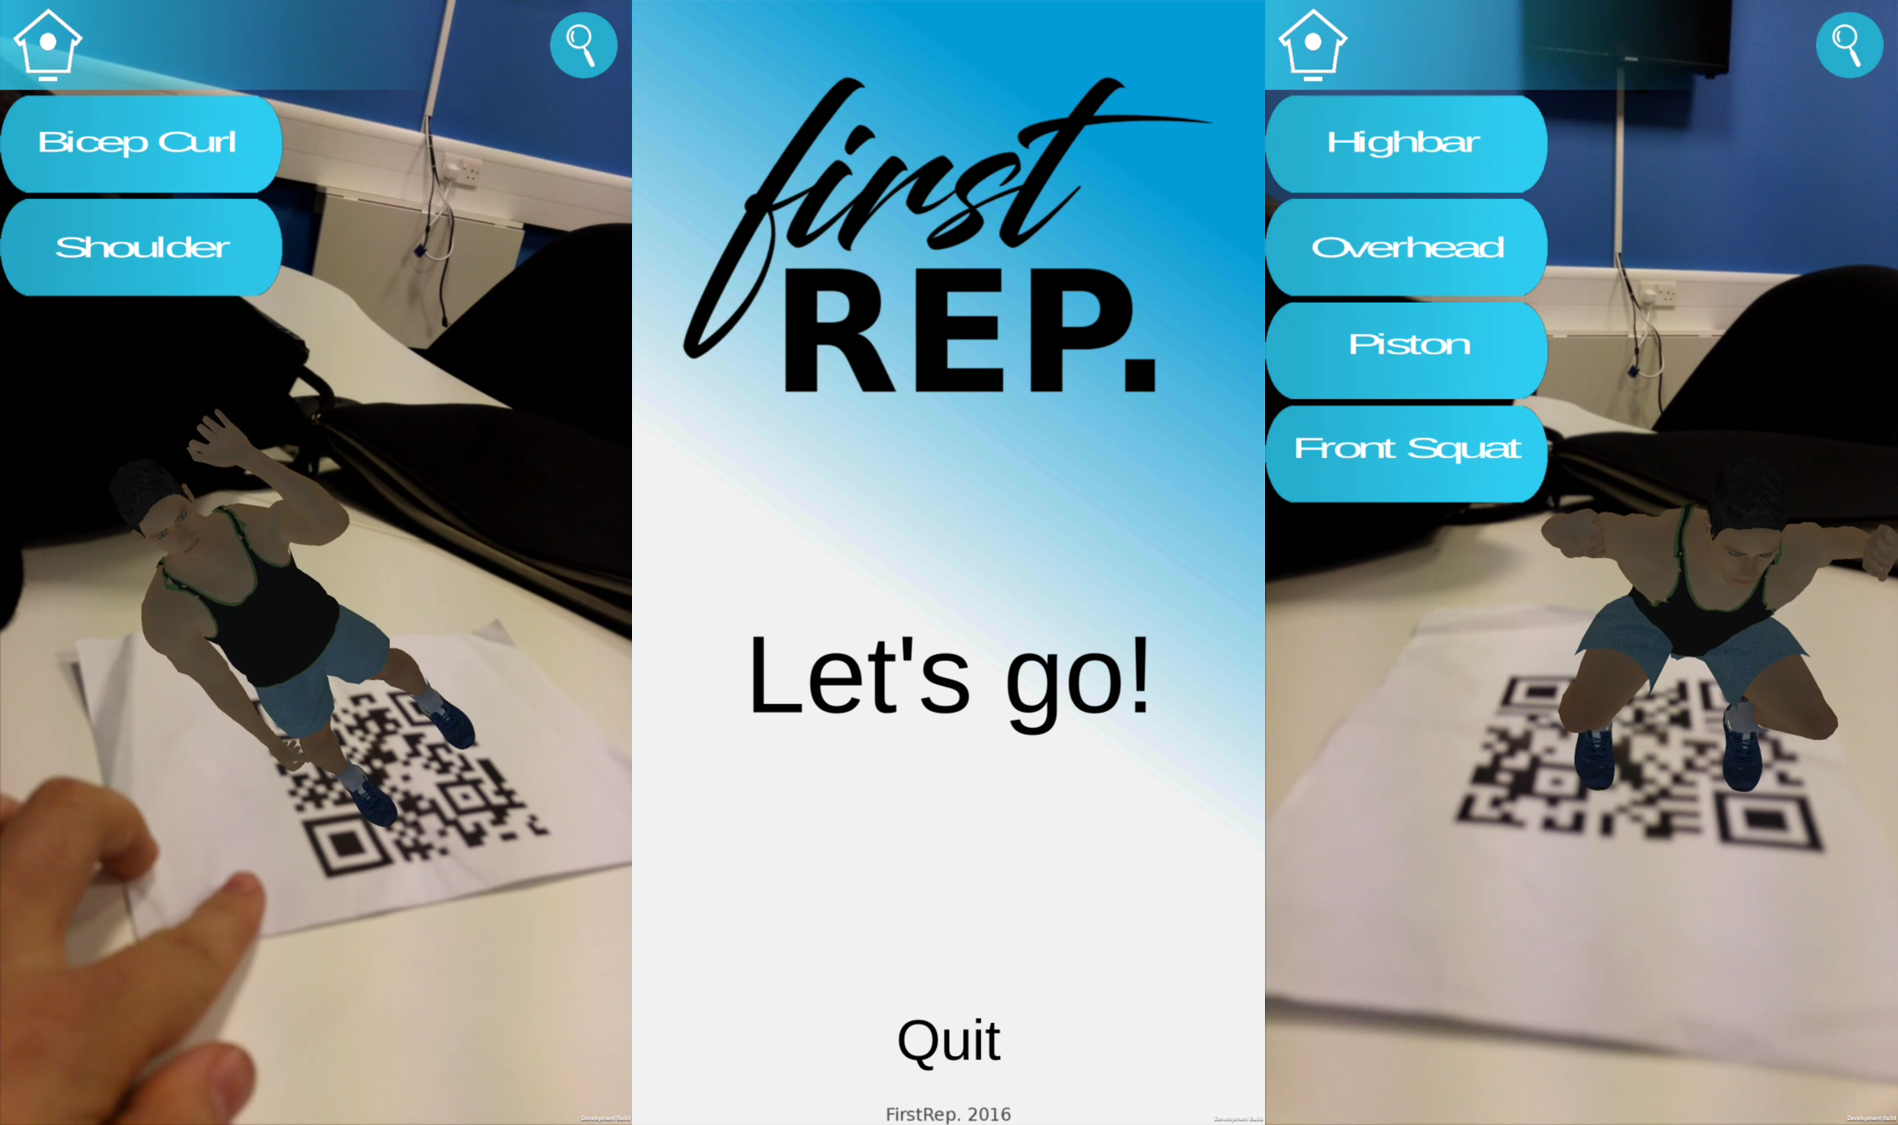
\includegraphics[width=\textwidth]{images/iteration1_screenshots.png}
\caption{Screenshots to show the state of the app at the end of the first iteration}
\label{fig:it1}
\end{figure}

Perhaps the most important outcome of the meeting was a reminder to the agreed upon size of the QR codes. In the initial meeting we discussed the QR codes being about the size of a postage stamp but so far during implementation I have simply been using large QR codes that take up about half a page of A4 paper simply because that is how they came out when I first printed them. I had completely lost track of the size and assumed I can simply shrink the QR code down when I need to however this is not the case. The actual sizing issue will be solved by simply adjusting the ration of QR code to avatar however there is a deeper issue here. By shrinking the QR code and making the avatar human size we will need the user to step back in order to fit the entire avatar into the screen view. It could be quite awkward for a user to have to come close to a machine, scan the QR code and then take a step back, all while pointing the phone in the correct direction. Furthermore, if the avatar appears right when the user scans the QR code, the user will be way too close and their entire screen will be filled by the avatar. It might be the case that we will have to calculate the distance between the user and the QR code and perhaps tell the user to step back until they are far enough to see the entire avatar - this could be potentially tricky and needs to be explored in the next phase of implementation. 

During the meeting, future functionality and possible extensions were also discussed. One feature that the president thought would be useful was a browse feature where you can group exercises by either equipment or target muscle group and then browse through them. When the user select an exercise, it will be rendered on the screen just like if the user triggered the exercise by scanning a QR code.

The topic of how the app could possibly be monetized also came up. While this is not the short term objective, nor is it a priority for now, it is important to consider options and make sure not to close any doors that could prove to be important in the long run. The option of a freemium model was discussed. A non-paying user would have access to a set of basic exercises and could download additional packs of exercises that are more advance or more specific. For example, a user could download a yoga package or an Olympic weightlifting package and thus expand the database of exercises that they have access to. This would not only be quite an effective way of generating income but it would also mean that packages of exercises can be rolled out in stages rather than having to do a significant amount of work before rolling out the app. In the long term, there is a lot of room for extra functionality. Features to log workouts, integrate with myFitnessPal or to download entire training programs are all feasible, however, these lie far beyond the scope of this paper and will thus not be discussed further here.

Overall, the GUSA president was quite impressed by app so far but was also aware of the fact that much more work is yet to be done. The meeting helped justify and confirm many of the design choices that I made. For example, the president and I agree on including equipment in the animations by default but having an option to toggle it on and off. We also agreed on having an about page which will explain how to safely use the app and then also have pop ups with safety disclosures that remind the user to stay safe and pay attention to their surroundings. Last but not least, we also discussed user testing and decided that this will take place in the Glasgow University Gym at the end of the next iteration.

\subsection{Second Iteration}
The intention of the second iteration was to act on some of the feedback that came from the meeting with GUSA and get the app ready for user trials.

\subsubsection{Redesign}
First impressions matter and in terms of software these impressions are often made through the design of the user interface. For the purpose of the first iteration, design was not a priority, ergo a redesign was due. The main focus of the redesign was the home page because that is what a user sees first and most frequently. As can be seen in figure \ref{fig:it1}, the initial design only had two buttons. Both buttons were plain text, with the top button taking the user to the AR camera and the quit button closing the application. During the redesign I decided to include more buttons and make them more obvious. This was both a design choice and a bi-product of the newly added info and search screens. The "quit" button was left out because android provides a hardware key to exit from applications and there is no need to duplicate the functionality. 

\subsubsection{Tracking}
The staple piece of functionality of the app is the tracking of markers and the display of animations in AR. The logic of how this functionality should work is relatively simple but it's implementations has proved to be quite challenging. The principle is to open up the camera and try to detect a marker that contains a specified pattern of features. Once we have acquired our target pattern, we display a 3D character, play an animation and then rotate,zoom and pan based on the movement of the phone. There are libraries such as Vuforia that abstract much of the heavy lifting to do with tracking markers and moving animations on screen, however they are not perfect. The single largest issue has been the detection and tracking of targets. Throughout development I have used markers that were roughly the size of half an A4 paper and had a character that was roughly the size of my palm so that I could test the app while sitting down next to the computer and wouldn't have to move around to fit the entire figure into view. My intention was to shrink the target and make the character proportionally larger by simply adjusting the reactions based on which the dimensions are calculated. While scaling up the character worked flawlessly, other unforeseen issues arose.

Having a small tracking target severely decreased the usability of the app because the user has to get close enough to the target for the camera to recognise it and then have to step back far enough to fit the entire figure into view. There are several problems with this. First, as the user is stepping back they are likely to move the phone around, thus moving the target out of view and loosing the tracking. Secondly, even if the user stands far back enough to see the entire figure, the target being used as an anchor is so small that recognizing it and it's exact orientation is difficult for the camera, causing flickering and misalignment. Lastly, the process simply involved too much movement which is not only inconveniently but also potentially dangerous. As a user is walking backwards and trying to keep the tracking active they may walk into objects or people behind them, risking injury.

\subsubsection{User Testing}
In order to assess the degree to which the application is fulfilling the set out requirements and objectives, user testing was carried out on the 18th of December 2016. The testing took place in Studio 1 of the Glasgow University Gym and participants were brought in individually to test the app. Each attendant was briefed concerning the privacy and anonymity of any collected information. Further, they were made aware that they may withdraw at any time or ask for their data to not be used. Each test consisted of two main parts. First the user was asked to use the app to carry out some possible user scenarios, which can be seen in figure \ref{test_scenarios}. The users were asked to speak out loud as they were thinking in order to identify any points of friction in using the app. Some trails were recorded using screen recording software. 

\begin{table}[h]
\centering
\caption{User scenarios used in testing}
\label{test_scenarios}
\begin{tabular}{ll}
1 & Find out how to do the piston squat.\\
2 & What exercises can be done at the curl station? \\
3 & Find the search page \\
4 & Find the info page \\
5 & What is the last station used for (referring to the deadlift platform)
\end{tabular}
\end{table}

The second part of the trial consisted of a short anonymous survey which the participant filled out without supervision. The questions asked in the survey can be seen in Appendix \ref{survey}. Results of the survey are summarized in Table \ref{survey_results}.

\begin{landscape}
\begin{table}[ht]
\centering
\resizebox{23cm}{!}{\begin{tabular}{p{2cm}p{2cm}p{2cm}p{2cm}p{2cm}p{2cm}p{3cm}p{3cm}p{2.9cm}}
Participant & Gender & Gym frequency & Design & Ease of use & Likelihood of future use & Best feature & Improvement Necessary & Further thoughts \\ \hline
A & M & 3 & 3 & 3 & 1 & You get to see the movements visually. & There could be text added to make it more informative. & N/a \\ \hline
B & M & 5 & 5 & 5 & 1 & Animations showing exercises & QR code allignment & Add more exercises and try to get a clearer animation view \\ \hline
C & F & 5 & 4 & 5 & 5 & Easy to use, very clear and helpful & The quality & Really good idea, would be very popular! \\ \hline
D & F & 5 & 5 & 4 & 5 & the idea in general, sometimes when you go to a new gym you dont know the new types of equipment, so this would really help & you need to learn to lean back rather than just tilting your phone, but once you understand that you need to do this it works really well & clever design \\ \hline
E & F & 1 & 3 & 5 & 4 & good use of qr & better visuals & so much potential for ad-ons \\ \hline
F & M & 4 & 5 & 5 & 5 & The full 3D animation allows you to see how to improve form accurately. & Probably keeping the animation up whilst walking around the QR code. & Would be very good for beginners as I personally would have loved to have had an app available to help me improve my form. \\ \hline
G & F & 3 & 4 & 3 & 4 & I liked being able to see the exercise from 360degrees. Makes it clear what to do :) & Stop it disapearing all the time & Would be good to see other (non-lifting) exercises - like yoga \\ \hline
H & M & 5 & 5 & 5 & 2 & Good for beginers & More exercises & Give more info on how to use the app \\ \hline
\end{tabular}}
\caption{User Scenarios used in testing}
\label{survey_results}
\end{table} 
\end{landscape}

Examining the data from the user testing we can see that the participants consisted of a mixture of male and female and had varying levels of experience in the gym, making our sample representative of the target audience. In the trial, the design of the app scored well, achieving a mean average of 4.25 out of 5. The users also found the app easy to use, giving it a cumulative average score of 4.375 out of 5. While these scores are encouragingly high, perhaps the most important metric - the likelihood of use, was quite low, scoring only 3.375 out of 5. What is more, the data is quite spread out and has a standard deviation of 1.77, which is significant in a scale of only 5. We can also observe a tendency for users who are frequent gym goers to be less likely to use the app (especially participants A,B \& H). This is likely due to the lack of variation in the exercises presented in the demo. These participants did not see the utility in using the app for experience gym goers since they already knew all the exercises demonstrated in the app. This claim is echoed in the qualitative user feedback with participants D, F \& H all stating that the app is "good for beginners" (Participant H). As a remedy, and to make the app more useful, some of the participants (A,B,E,G \& H) suggested adding more exercises as the single most important improvement. Participant E identified the opportunity for having add-ons in the form of workout packs and Participant G commented that the app could be used to demonstrate yoga exercises. Contemplating this feedback has brought up the idea to provide a \textit{freemium} service where every user receives a basic set of exercises and can pay to download additional packs of exercises that are grouped together by a common theme such as yoga, Olympic weightlifting or stretching. For the purpose of this report a small sample of yoga exercises will be created to demonstrate the variety of exercises that could be made available. 

Coming back to the user data in Table \ref{survey_results}, we can see the design of the application was received well but some issues were identified in the qualitative feedback. All participants, except H, commented on the usability, alignment or quality of animations in the app. During usage, many users struggled to keep the animation tracking because as they moved around they would loose the QR code from the viewport and the animation would disappear. This is clearly an area of improvement. As Participant D pointed out, "you need to learn to lean back rather than just tilting your phone, but once you understand that you need to do this it works really well". Therefore a possible solution would be to include a prompt on first use which instruct the user how to track with the phone in such a way that the animation is not lost. Perhaps a better option would be to configure the tracking to not disappear if the marker is lost in the y-axis. Thus, if the user pans up and down with the device, the animation stays rather than disappears due to the marker being bellow the field of view. 

Making information about how to perform exercises is the principal objective of the app and therefore I decided to implement a browse view where users could scroll thought the different exercises categorized by either muscle group or equipment. When I began developing the functionality I realised that having a browse view could be quite confusing in an augmented reality application. I therefore halted development of this function and create a quick prototype version of it instead. I then used the user testing as an opportunity to collect user opinion to inform my decision. The majority of users thought the browse function was a good idea and were able to navigate to it in the app and understand it's purpose. I asked the user what they expect to happen when they click on an exercise in the browse view and almost all users wanted to see the animation of the exercise appear on screen (even though there is no marker). This animation would not track along with the sideways movement of the phone but would be able to rotate as the phone pans. It is likely that such functionality will be implementable given the technologies available however confirmation is pending further investigation. 

\subsection{Third Iteration}
\subsubsection{Tracking}
\subsubsection{Search}


\chapter{Conclusion}

\chapter{Evaluation}

%\vspace{-7mm}
\begin{figure}
\centering
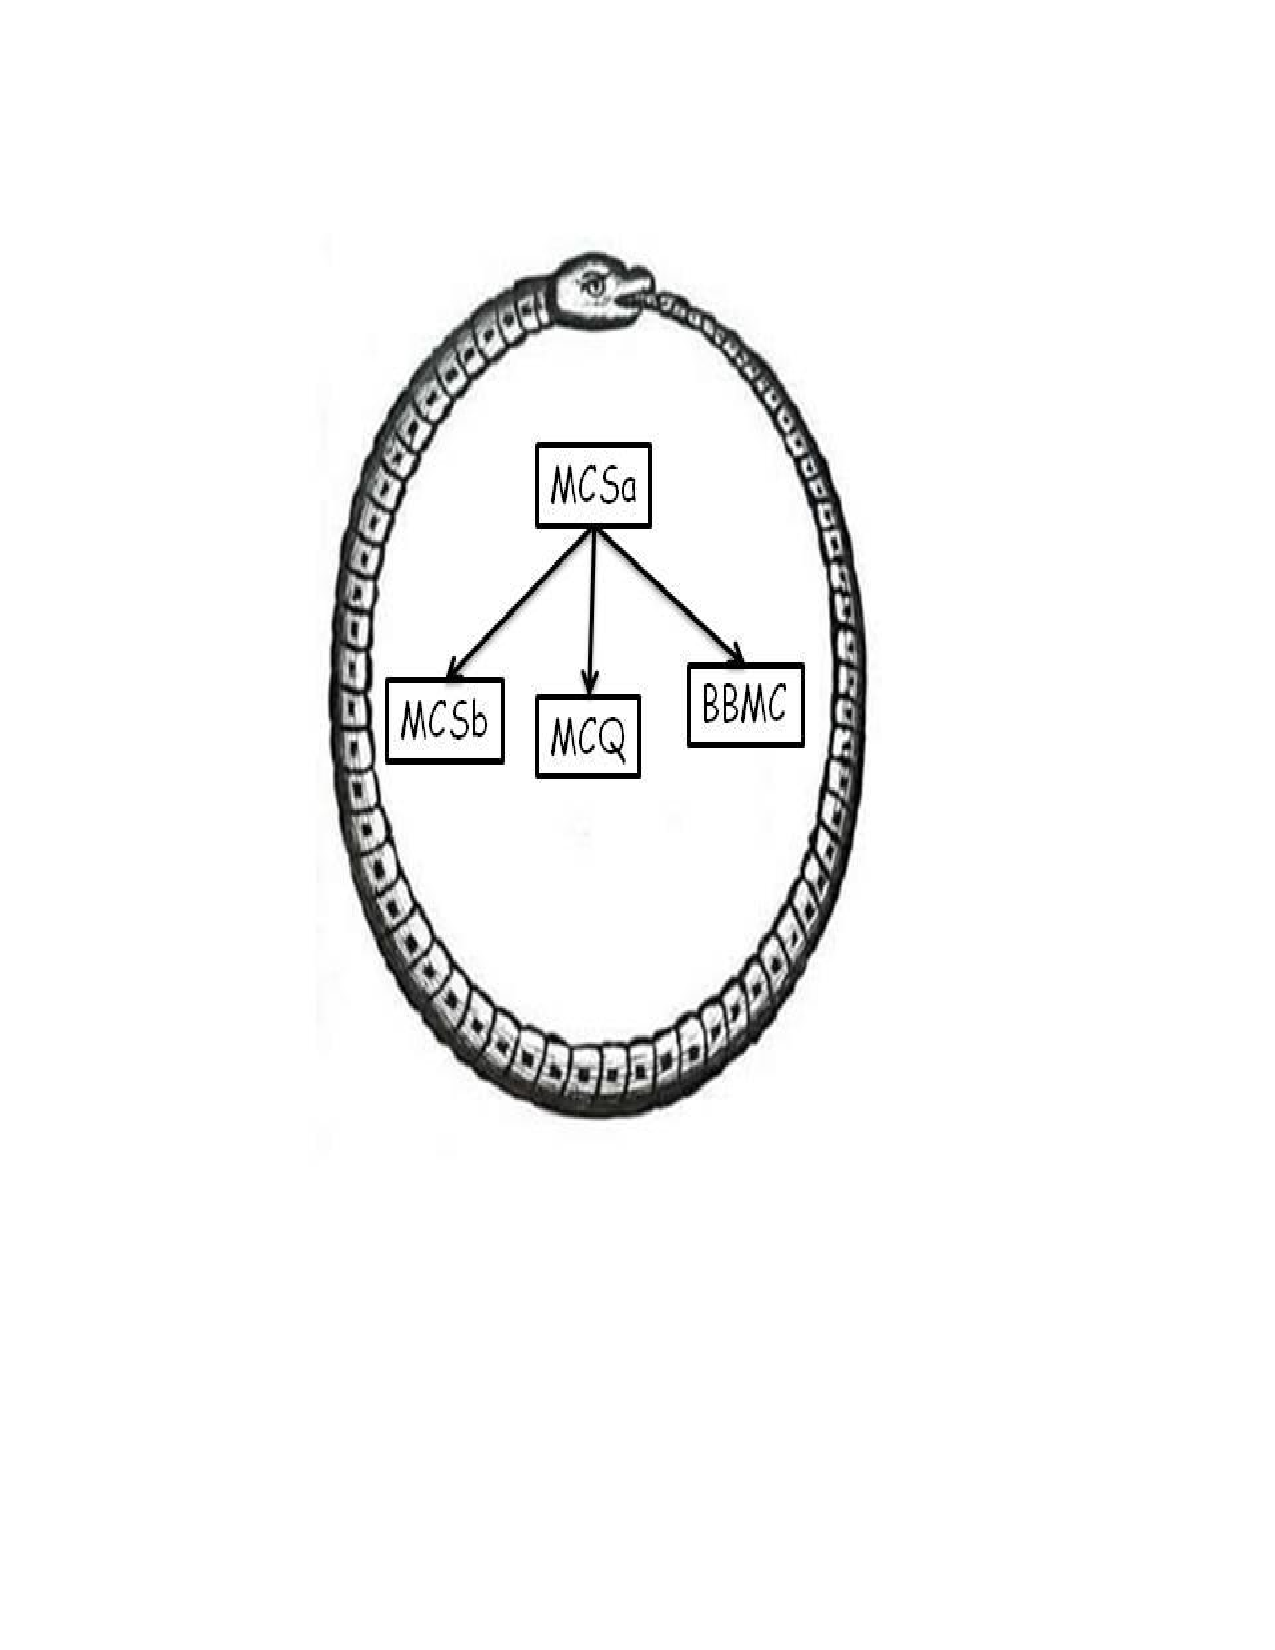
\includegraphics[height=9.2cm,width=13.2cm]{uroboros.pdf}
\vspace{-30mm}
\caption{An alternative hierarchy of the algorithms.}
\label{uroborus}
\end{figure}



%%%%%%%%%%%%%%%%
%              %
%  APPENDICES  %
%              %
%%%%%%%%%%%%%%%%
\begin{appendices}
\chapter{User Testing Survey}
\label{survey}
\textbf{Question 1:} Gender \\
\textbf{Option(s):}    Male, Female, Prefer not to answer
\\
\\
\textbf{Question 2:} How often do you go to the gym? \\
\textbf{Option(s):}    Scale from 1 to 5 (Never - Every day)
\\
\\
\textbf{Question 3:} What do you think of the design? \\
\textbf{Option(s):}    Scale from 1 to 5 (Horrible - Awesome)
\\
\\
\textbf{Question 4:} How easy is the app to use? \\
\textbf{Option(s):}    Scale from 1 to 5 (Very Difficult - Very Easy)
\\
\\
\textbf{Question 5:} How likely would you be to use the app? 
\\
\textbf{Option(s):}    Scale from 1 to 5 (I wouldn't - I definitely)
\\
\\
\textbf{Question 6:} What is the best thing about the app? \\
\textbf{Option(s):}     Any answer.
\\
\\
\textbf{Question 7:} What needs to be improved the most?? \\
\textbf{Option(s):}     Any answer.
\\
\\
\textbf{Question 8:} Any further thoughts?? \\
\textbf{Option(s):}     Any answer.

\chapter{Running the Programs}
An example of running from the command line is as follows:
\begin{verbatim}
      > java MaxClique BBMC1 brock200_1.clq 14400
\end{verbatim}
This will apply $BBMC$ with $style = 1$ to the first brock200 DIMACS instance allowing 14400 seconds of cpu time.

\chapter{Generating Random Graphs}
\label{sec:randomGraph}
We generate Erd\'{o}s-R\"{e}nyi random graphs $G(n,p)$ where $n$ is the number of vertices and
each edge is included in the graph with probability $p$ independent from every other edge. It produces
a random graph in DIMACS format with vertices numbered 1 to $n$ inclusive. It can be run from the command line as follows to produce 
a clq file
\begin{verbatim}
      > java RandomGraph 100 0.9 > 100-90-00.clq
\end{verbatim}
\end{appendices}

%%%%%%%%%%%%%%%%%%%%
%   BIBLIOGRAPHY   %
%%%%%%%%%%%%%%%%%%%%

\bibliographystyle{plain}
\bibliography{bib}

\end{document}
